\chapter{Approach} % (fold)
\label{cha:approach}
\headermark{approach}

\section*{} % (fold)
The proposed approach consists in envisioning scaling and performance optimization as a whole, where all components take part in scaling and improving the system. Having that said, it is necessary to look out for sensitive dependencies, or the aforementioned \textit{butterfly effect} when optimizing the system.

As an example, the Ruby MRI interpreter's garbage collector consists in an implementation of the \textit{mark-and-sweep} algorithm which is good enough for most applications but lacks the efficiency to deal with heavy and memory intensive applications like Rails~\cite{passenger_whatis}. It is a perfectly reliable garbage collector for the majority of Ruby applications, but it is not the best choice for Rails itself.

Every component must be seen from the Rails perspective and bottlenecks must be identified and contoured.

To achieve this, we need to set up an initial setup for benchmarking, tweaking and patching. This involves using a specific operating system and that choice will be made based on three essential factors:
\begin{enumerate}
  \item The information gathered in the state of the art of Operating Systems, from the Rails perspective;
  \item A small set of benchmarks for standard performance analysis;
  \item Configuration easiness, as some operating systems and distributions tend to stimulate system tweaking by allowing easy access to certain features and configurations and others, on the other hand, might not have this feature in their goals and consequently make it harder to tweak and configure at will.
\end{enumerate}
After starting with the chosen operating system, kernel settings will fill the first chapter of the abovementioned guidelines as they have a great impact on operating system behavior. Important settings regarding TCP/IP behavior, I/O scheduler, Preemption, Interrupt Timers \textit{et al.} must be tested and benchmarked from the Rails perspective in order to achieve a configuration set that suits Rails --- and all the other components --- best.

When the mentioned set of configurations and settings is met, the web servers will become the research and development target. Not all of them will be tested since the state of the art on web servers rules some of them out, but at least two will be taken into a small set of benchmarks and configuration tweaking. After finding which suits Rails best, research will deepen and eventual bottlenecks might be found and improving patches will be developed.

Following the web server choice, ruby interpreters will become the aim. Once again, the state of the art on ruby interpreters rules some of them out but at least two will endure a small set of benchmarks and configuration tweaking to conclude which scales better and has a better performance from the Rails point of view. Possible bottlenecks will be found and, once again, an attempt at solving the most critical ones will be made. After that, a series of patches will be released in order to improve that interpreter even further.

The next target is a commonly know bottleneck on web applications – the database. A few will be tested, following the \textit{at least two} rule, but here there is a clear division on two essential types of databases:
\begin{enumerate}
  \item Schema-based databases, like the famous MySQL or PostgreSQL;
  \item Schema-free document-oriented databases, like MongoDB or CouchDB.
\end{enumerate}
While schema-based databases are very popular and reliable, not to mention that they are tested thoroughly because of being so popular and so mature, schema-free databases emerge as high performance solutions with little pitfalls. Both types must be tested and benchmarked, in order to provide results and configurations that suit most Rails applications, whether they are using a schema-based database or not. Bottlenecks will also be searched and attempts at fixing them will be made. An approach to caching will also be made in the database regard, as it is a crucial concept when scaling. If major bottlenecks are found in the existing caching solutions, an improvement attempt will be made and possible positive outcomes will be submitted as patches to the developing community.

The next phase is related to Rails itself. Since, as mentioned, Rails 3.0 is a big improvement over Rails 2.3 from a performance perspective, no attempts at improving Rails 2.3 will be made. However, remaining bottlenecks in Rails 3.0 will be targeted for improvement with guidance from the Rails core development team.
Finally, the case-study application, Escolinhas~\cite{escolinhas}, will be aimed for improvement. The architecture and code will be reviewed to find and erase performance bottlenecks, always taking Rails' strengths and weaknesses into account to fully optimize the application for the framework it is being developed on. This will allow the development of a small set of generalist guidelines and programming conventions that suit most Rails developers and their respective applications.
Different components become the main focus at different times. A brief summary of the above information is presented in table~\ref{tab:research_development_schedule} which indicates when a given component will become the main focus and for how long that is expected to happen.
\begin{table}[h]
  \centering
  \begin{tabular}{p{8cm}|p{2.1cm}p{3.5cm}}
    \textsc{Target component}
  & \textsc{Start date}
  & \textsc{Duration (weeks)}
  \\
  \hline
    \textbf{OS Choosing}
  & 15/02/2010
  & 1
  \\
  \hline
    \textbf{OS kernel testing and tunning}
  & 22/02/2010
  & 1
  \\
  \hline
    \textbf{Web server testing and bottleneck research}
  & 01/03/2010
  & 1
  \\
  \hline
    \textbf{Web server bottleneck improvements}
  & 08/03/2010
  & 1
  \\
  \hline
    \textbf{Ruby interpreter testing and bottleneck research}
  & 15/03/2010
  & 1
  \\
  \hline
    \textbf{Ruby interpreter bottleneck improvements}
  & 22/03/2010
  & 1.5
  \\
  \hline
    \textbf{DB testing and bottleneck research}
  & 31/03/2010
  & 1
  \\
  \hline
    \textbf{DB bottleneck improvements}
  & 07/04/2010
  & 1
  \\
  \hline
    \textbf{Rails 3.0 bottleneck research}
  & 14/04/2010
  & 1
  \\
  \hline
    \textbf{Rails 3.0 bottleneck improvements}
  & 21/04/2010
  & 2.5
  \\
  \hline
    \textbf{Escolinhas analysis and bottleneck research}
  & 10/05/2010
  & 1
  \\
  \hline
    \textbf{Escolinhas platform improvements}
  & 17/05/2010
  & 3
  \\
  \hline
    \textbf{Write dissertation report}
  & 07/06/2010
  & 4
  \\
  \end{tabular}  
  \caption{Component focus scheduling}
  \label{tab:research_development_schedule}  
\end{table}\\
In order to benchmark every component, others which run on top of it must be taken into account. This way, the research starts by involving every single component. After having conclusive results for each one of them they will be removed from the research, as shown on figure~\ref{fig:gantt}. The main focus will then leap into another component.
\begin{figure}[th]
  \begin{center}
    \leavevmode
 
    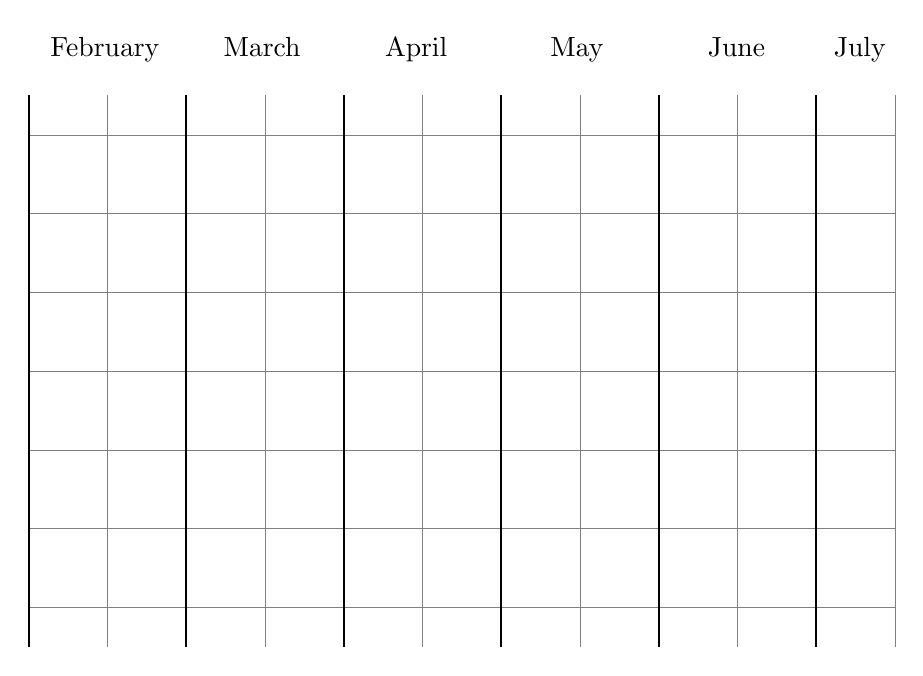
\begin{tikzpicture}[y=-1cm]
      \draw[help lines] (0,7.5) grid (11,0.5);
      \draw[thick] (0,0.5) -- (0,7.5);
      \draw[thick] (2,0.5) -- (2,7.5);
      \draw[thick] (4,0.5) -- (4,7.5);
      \draw[thick] (6,0.5) -- (6,7.5);
      \draw[thick] (8,0.5) -- (8,7.5);
      \draw[thick] (10,0.5) -- (10,7.5);
      
      \node at (0.15,0.0) [anchor=base west] {February};
      \node at (2.35,0.0) [anchor=base west] {March};
      \node at (4.4,0.0) [anchor=base west] {April};
      \node at (6.5,0.0) [anchor=base west] {May};
      \node at (8.5,0.0) [anchor=base west] {June};
      \node at (10.1,0.0) [anchor=base west] {July};
      
      \ganttline{1}{Operating Systems}{15}{30}
      \ganttline{2}{Web servers}{22}{37}
      \ganttline{3}{Ruby interpreters}{22}{55}
      \ganttline{4}{Databases}{22}{70}
      \ganttline{5}{Ruby on Rails}{22}{95}
      \ganttline{6}{Escolinhas}{22}{125}
      \ganttline{7}{Thesis Writing}{125}{155}
    \end{tikzpicture}
 
    \caption{Work scheduling}
    \label{fig:gantt}
  \end{center}
\end{figure}\\
All the mentioned testing, tuning, bottleneck research and improvements are directly related to scaling and performance optimizations, as suggested throughout this thesis.
Once again, it becomes critical to reaffirm that each area will be essentially targeted from the Rails perspective, taking sensitive dependences into account in order to avoid optimizing a specific component while taking the risk of making the system, as a whole, slower or less scalable.

